\documentclass{article}

% Language setting
% Replace `english' with e.g. `spanish' to change the document language
\usepackage[english]{babel}

% Set page size and margins
% Replace `letterpaper' with `a4paper' for UK/EU standard size
\usepackage[letterpaper,top=2cm,bottom=2cm,left=3cm,right=3cm,marginparwidth=1.75cm]{geometry}
\usepackage{listings}

% Useful packages
\usepackage{amsmath}
\usepackage{graphicx}
\usepackage{subfig}

\usepackage[colorlinks=true, allcolors=blue]{hyperref}

\title{3D Shape, Pre-processing and Visualization}
\author{Megan Mirnalini Sundaram R, Sherry Usman}

\begin{document}
\maketitle



\section*{Question 1}
\subsection*{Slices and Aspect Ratio}
The image has 16 slices. The aspect ratio can be defined as the ratio of total width (total number of columns) and the total height (total number of rows). In that case it is 160/140 which is 1.143. 

\subsection*{Function to display the contents of the 3D image}
The code snippet below shows the function for displaying the slices of the image.  
\begin{lstlisting}
import numpy as np
import matplotlib.pyplot as plt 

num_slices = 16
fig, axes = plt.subplots(4,4, figsize =(12,12))
for i in range(num_slices):
  ax = axes[i // 4, i % 4]
  tif.seek(i)
  slice = np.array(tif)

  ax.imshow(slice)
  ax.axis('off')
  ax.set_title(f'Slice {i+1}')

plt.tight_layout()
plt.show()
\end{lstlisting}


\section*{Question 2}
We applied thresholding on the chromo.tiff image using the diplib library in Python and using VAA3D software. Figure \ref{fig:otsu-median} shows the result of the Otsu Threshold (left) and the result of Otsu threshold with median filter (right). 

\begin{figure}%
    \centering
    \subfloat[\centering label 1]{{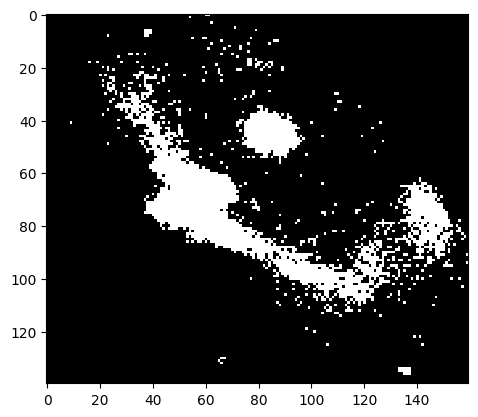
\includegraphics[width=0.45\textwidth]{Report/Images/otsu_threshold_image.png} }} \label{fig:Otsu}%
    \qquad
    \subfloat[\centering label 2]{{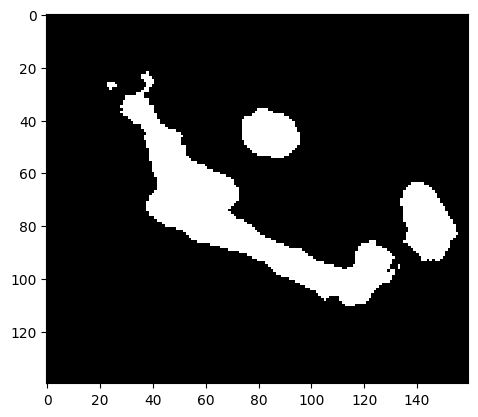
\includegraphics[width=0.45\textwidth]{Report/Images/median_filter.png} }}%
    \caption{Chromo.tiff with otsu threshold (left) and median filter and otsu threshold (right)}%
    \label{fig:otsu-median}%
\end{figure}

Figure \ref{fig:vaa3dthresh} shows the result of the VAA3D software. As seen in figure \ref{fig:vaa3dthresh} the best threshold value is 55. 

\begin{figure}
    \centering
    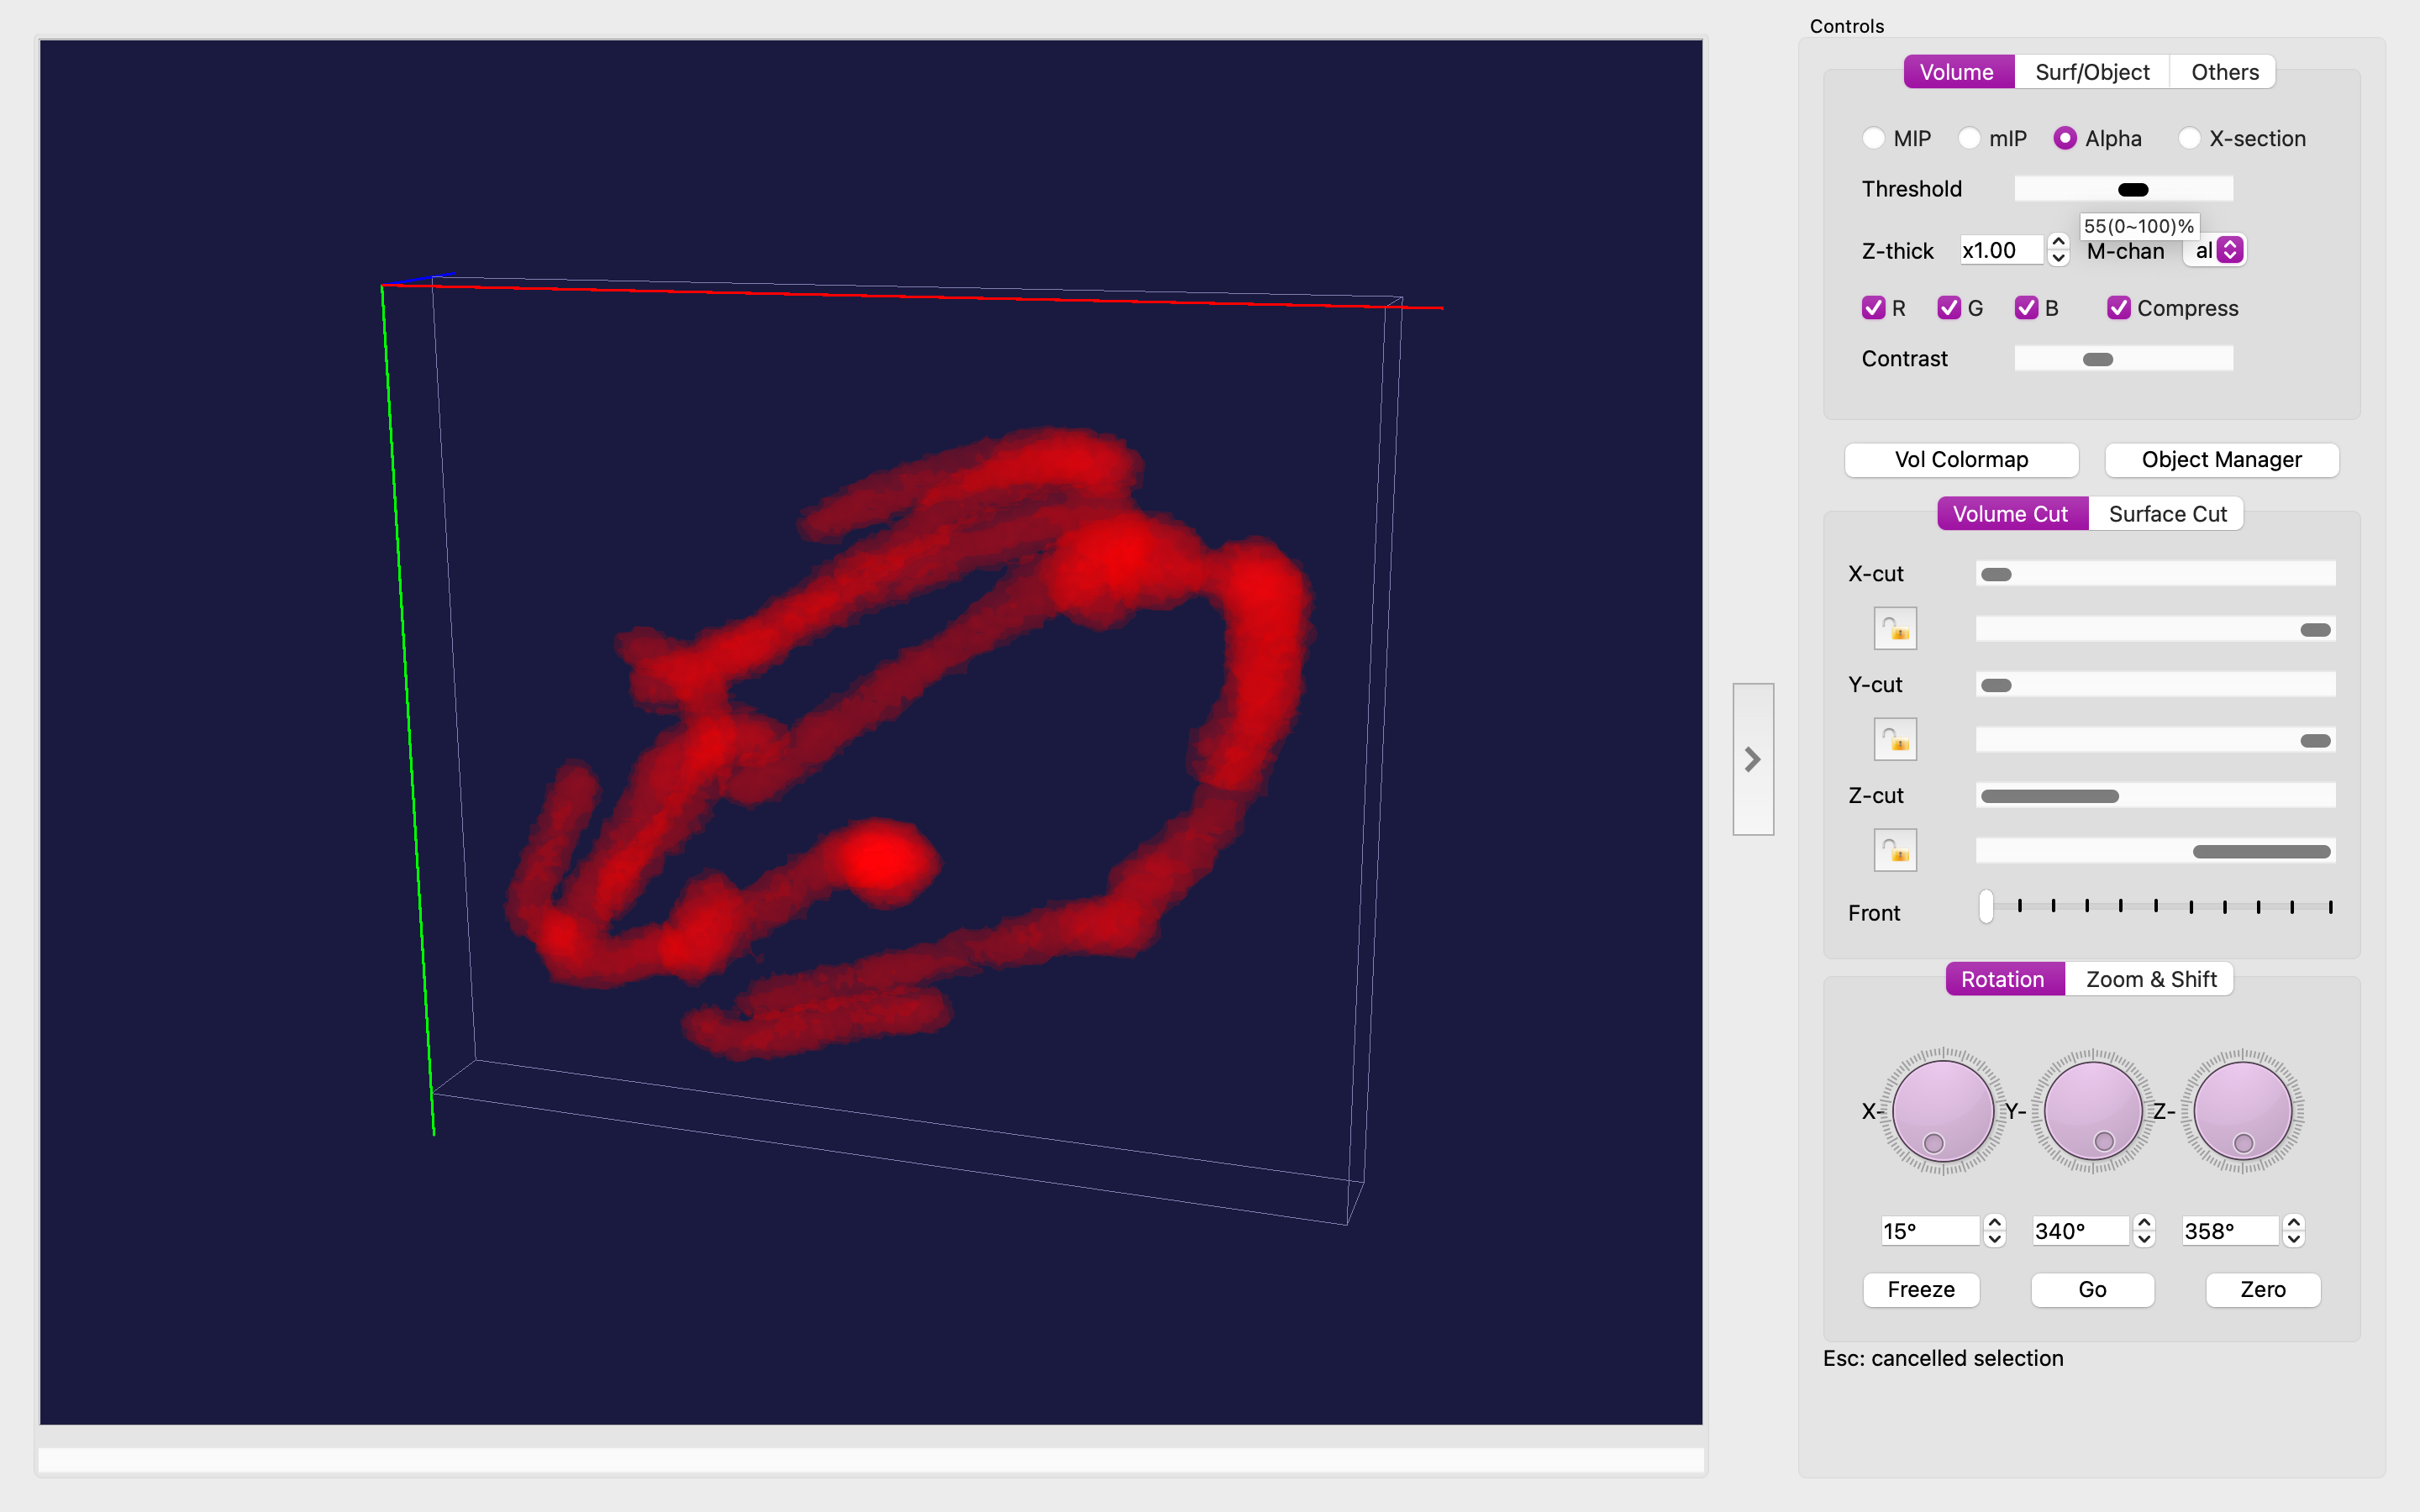
\includegraphics[width=1\linewidth]{Report/Images/vaa3d_thresh.png}
    \caption{Chromo.tiff image thresholded in VAA3D}
    \label{fig:vaa3dthresh}
\end{figure}

\section*{Difference Between Figure 1 and 2}

The first image is a raw image obtained before processing techniques such as thresholding, median filter and contrast stretching. Thus it looks out of focus, blurry and underexposed. The second image is the product of these image analysis methods and the original image. 



\bibliographystyle{alpha}
\bibliography{sample}

\end{document}